\chapter{Modernising Rate Monitoring Tools}

One of the major challenges for the Compact Muon Solenoid (CMS) experiment, is the task of reducing event rate from roughly 40 MHz down to a more manageable 1 kHz while keeping as many interesting physics events as possible. This is accomplished through the use of a Level-1 (L1) hardware based trigger as well as a software based High-Level Trigger (HLT). Monitoring and understanding the output rates of the L1 and HLT triggers is of key importance for determining the overall performance of the trigger system and is intimately tied to what type of data is being recorded for physics analyses.

Here, we introduce the Trigger System in operation at the CMS experiment and proceed giving an overview of the software development work done to improve and add new features to the CMS Rate Monitoring software, a collection of tools used by CMS shifters to monitor the L1 and HLT trigger rates. Some other experimental components have ben developed to showcase possible upgrades, delivering quality of life enhancements and enabling shifters and physicists to navigate data in a faster and more comfortable way.

Finally, proper export functionalities have been added to the tools, allowing to save and export Trigger Rates as JSON or ROOT binary files.

This work is also described in \cite{VivaceRTM1} \cite{VivaceRTM2} \cite{L1TriggerOMSDevelopments} \cite{MohrmanRTM}, the source code is available in the RateMon git repository \cite{RateMonGit}.

\section{CMS Trigger System}

A Trigger is an  electronic system for spotting potentially interesting collisions in a particle detector and triggering the detector’s read-out system to record the data resulting from the collision.

The LHC generates 40 millions events per second. Each event recorded by the CMS detector, carries on average a payload of 1 MB of unprocessed informations. It is technologically impossible to retain this amount of data, due to hardware, software, network and storage constraints. Furthermore, most events represent uninteresting information for the current state of physics knowledge.

The \textit{CMS Trigger System} is designed to reduce the output stream to 1000 events per second, while preserving the physics reach of the experiment.
It is composed by a hierarchical set of rules, called Trigger Nodes (or Paths): each one probes a specific patterns (physics signature) in the event or looks for specific physics objects.

This happens in two steps:

\begin{enumerate}

    \item The first level (L1) \cite{Bayatyan:706847} brings the 40 MHz to a 100 kHz rate. Here, N Trigger Algorithms are implemented on custom electronics (FPGAs and ASICs) exploiting informations from sub-detector components.

    \item A configurable set of L1 Trigger Nodes seeds Triggers in the second level (HLT), implemented in software. The event stream is further refined, selecting an average rate of 400 Hz for offline event storage and certification \cite{Khachatryan_2017}. HLT runs 600 of these independent Trigger Paths.

\end{enumerate}

\begin{figure}
    \centerline{
        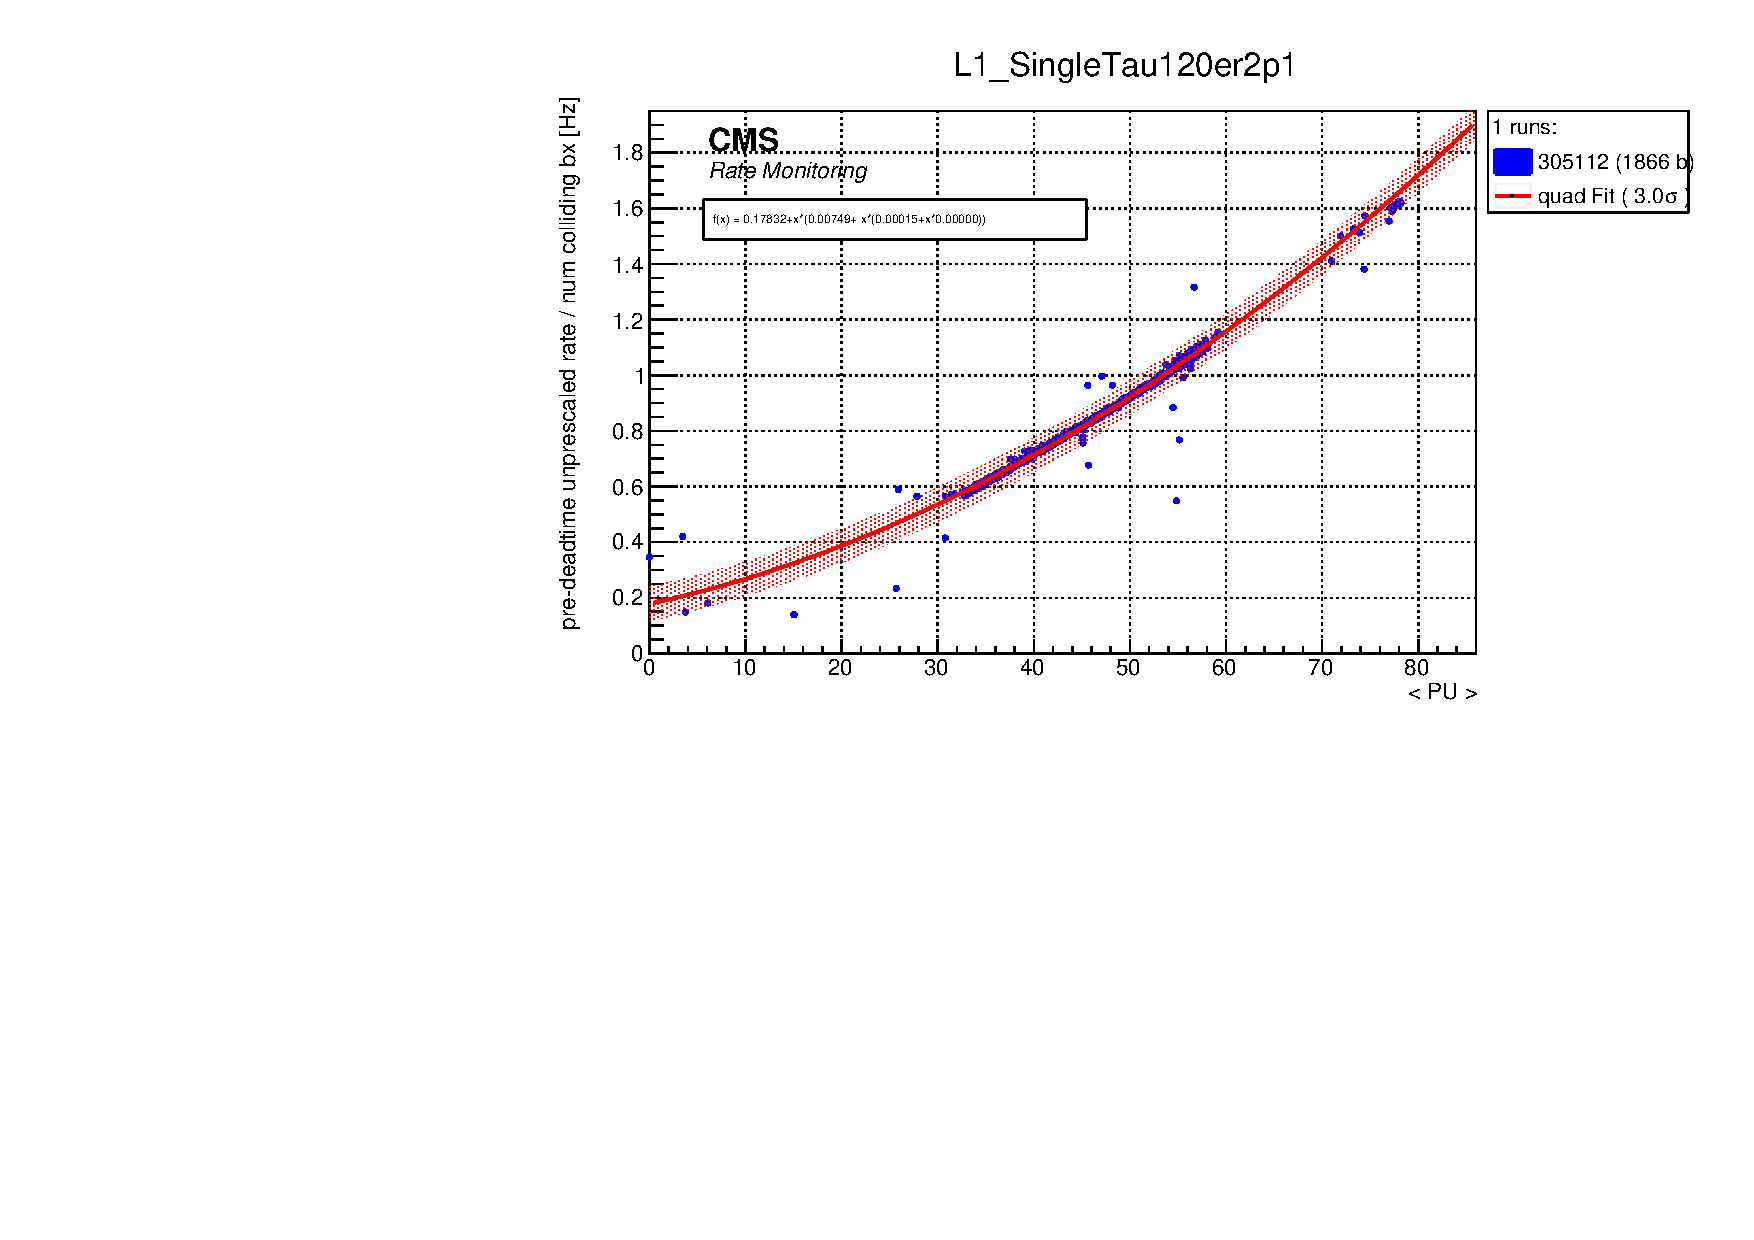
\includegraphics[width=0.6\paperwidth]{figures/RMT_305112_L1_SingleTau120er2p1.pdf}}
    \caption{L1 Trigger path plotted with a fitted function on run 305112}
    \label{fig:ratemon_l1}
\end{figure}

\begin{figure}
    \centerline{
        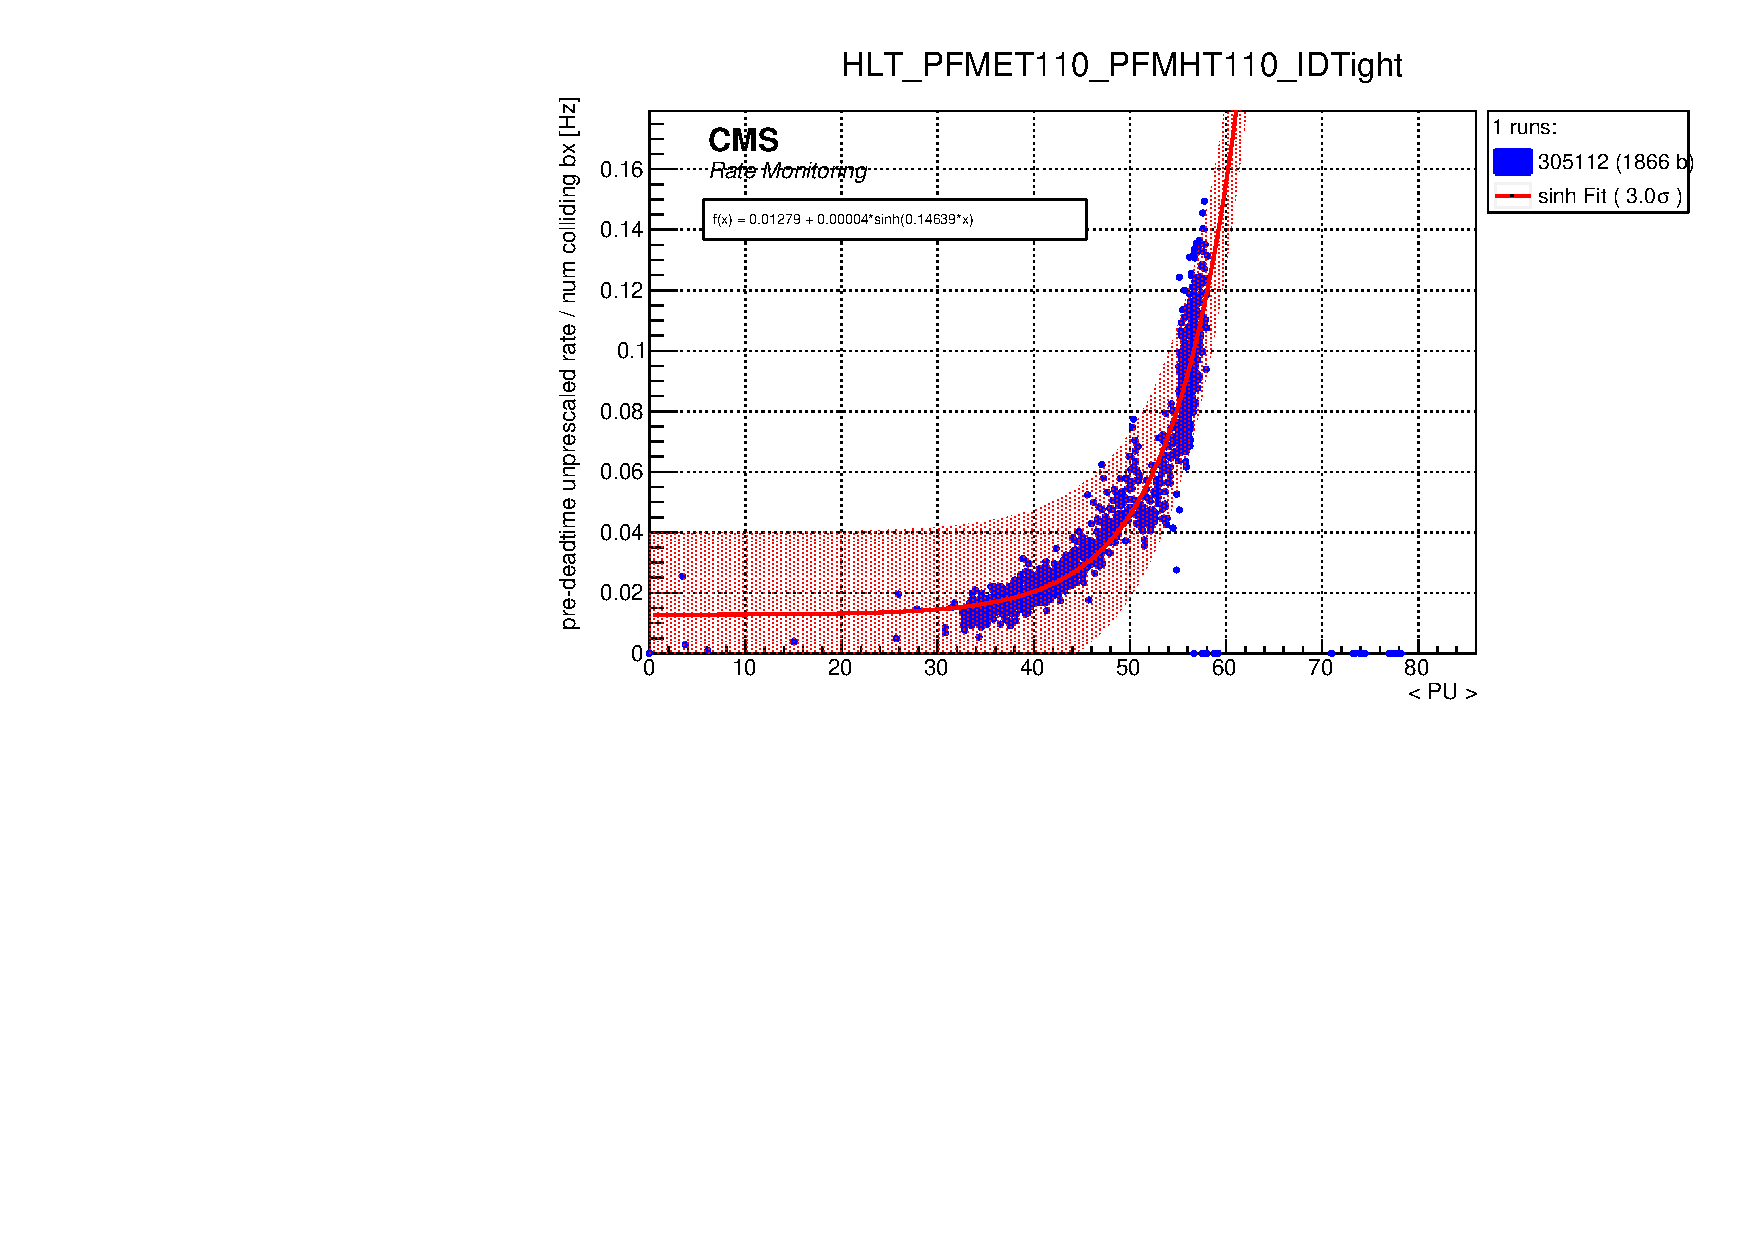
\includegraphics[width=0.6\paperwidth]{figures/RMT_305112_HLT_PFMET110_PFMHT110_IDTight.pdf}}
    \caption{HLT Trigger path plotted with a fitted function on run 305112}
    \label{fig:ratemon_hlt}
\end{figure}

\section{Rate Monitoring software}

\subsection{Shift Monitor tool}

The High Level Trigger (HLT) rate monitoring tool is a python script that reports the rates of a selected list of triggers, primary datasets, and streams. It is run in the CMS control room and gives valuable real-time feedback of trigger rates to the shift crew: it updates every minute and averages the rates recorded in the last 3 lumisections, and, if possible, compares them to the predicted rate. If a trigger path deviates by a specified amount from the prediction, or exceeds a fixed rate, the corresponding line is highlighted in a yellow colour. The scripts also displays other information that could be useful for the shifter, such as the run number and last lumisections, the LHC status, HLT key, deadtime, instantaneous luminosity and index of the prescale column in use.

\begin{figure}
    \centerline{
        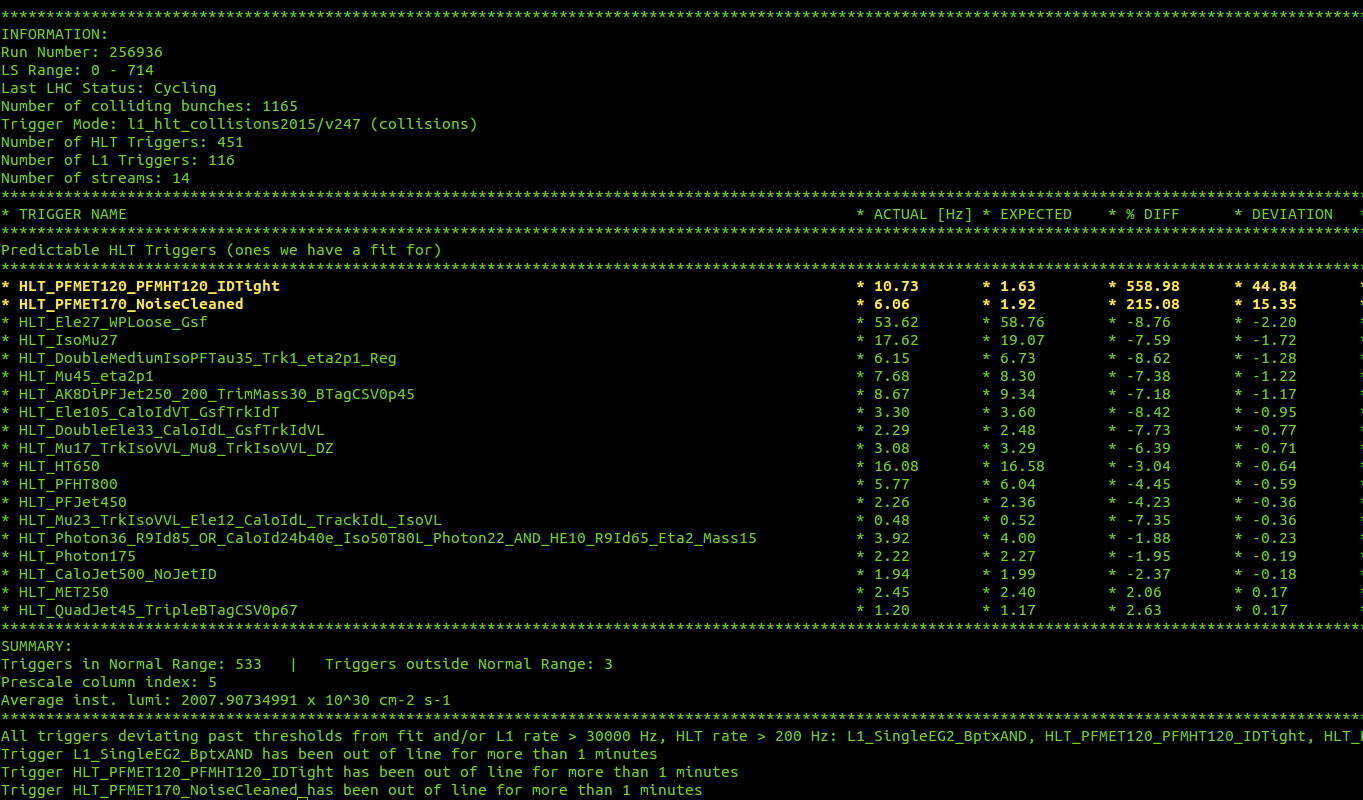
\includegraphics[width=0.8\paperwidth]{figures/ratemon_warnings}}
    \caption{Example execution of the Rate Monitoring Tool showing warnings: two triggers have values consistently deviating from the predictions. \cite{ratemon-twiki}}
    \label{fig:ratemon_warnings}
\end{figure}

\subsection{Trigger Rate plotting}

Another part of the software is plotting library, exposed as a the \texttt{plotTriggerRates} command line tool: it is used for observing how trigger rates vary over a range of beam and detector conditions, in particular how the rates of individual triggers scale with event pile-up.

Trigger Rates are usually represented in \textit{Rate vs. PileUp plots}, specifically "pre-deadtime unprescaled rate / num colliding bx [Hz]" over "PU" (Pile Up luminosity) units, generated by the RateMon tools.

In general, \textit{deadtime} refers to a time period during normal data taking when collisions are occurring but CMS is not ready to record the the data. This can occur for various reasons that are described in section 6.2.1 of \cite{Khachatryan_2017}. "pre-deadtime" rates are used in plots to allow for consistent comparison between different runs/fills; different runs and fills could have had different deadtimes, so correcting the rates for deadtime before fitting will allow the rates from different runs to be compared in a consistent way.

A \textit{prescale} is a way of scaling back the rate of L1 and HLT triggers. For example, if a certain trigger has a prescale of 5, then the data corresponding to the event the trigger fired on is only recorded once out of every five times that the trigger fired. So if the prescale is 1, the data will be recorded every time the trigger fires. A prescale of 0 actually means that no data will be recorded for the trigger in question; the trigger is essentially just turned off. Again, correcting for deadtime in Rate VS PU plots is to allow for consistent comparisons of rates for different runs/fills and across pre scale columns. 

\section{Packaging, CI/CD}

To enable CI/CD, we moved the repository on the CERN GitLab. The repository on GitHub is being kept updated but the CI/CD is handled by GitLab.
I've restructured the folder. The "misc" folder now contains the fits logs and the wbmRateReader. The ratemon folder is the only one actually being packaged. The "systemd" folder contains the service file allowing the \texttt{ShiftMonitorTool} to be installed and used as a systemd service.

Docker, GitLab ci, cernbox

Each commit triggers a build and a deployment of a RPM package. This CI/CD system is configured in these files:

\begin{enumerate}
    \item \texttt{.GitLab-ci.yml} describes the GitLab CI. The first phase (\texttt{build\_rpm}) tells the builder (described by \texttt{builder.dockerfile} and exposed on the GitLab registry) to run \texttt{make rpm} (described in \texttt{Makefile}) and flags the RPM package files as artifacts; In the second phase (deploy), those artifacts are pushed on a EOS folder using the ci-web-deployer tool;
    \item \texttt{builder.dockerfile} prepares the docker container that will run the build, starting from the cern/cc7-base image. This is exposed using the GitLab registry feature as \texttt{gitlab-registry.cern.ch/avivace/ratemon/builder};
    \item \texttt{Makefile} Uses the fpm tool to produce an RPM file with the given metadata and contents. Basically, the ratemon script folder is copied into /opt/ and the systemd service file goes into /usr/lib/systemd/system
    \item The build produces an RPM package file. Those files are pushed during the "deploy" CI phase and finally published on a public CERNBox folder (EOS: \texttt{/eos/users/a/avivace/ratemon\_builds}). This is done using a service CERN account.
\end{enumerate}

Previously, the RateMon tools had to be installed checking out the code from the git repository, running a preparatory script, configuring the database connection and then running the script. Now, the system package manager can install the packaged software.

\subsection{CMS Cactus}

CMS Cactus auto devops \cite{DirkxCactus} is a collection of GitLab CI templates and images designed to ease development and maintenance of CI workflows for Cactus projects. It is built on the same foundations as GitLab AutoDevOps, but tailored for CERN and CMS infrastructure.

We moved the CI/CD and packaging pipeline from vanilla’s GitLab tools to CMS Cactus, now using (and customising) a template provided by this tool.

TODO improvements, examples

\begin{listing}[ht]
\begin{yamlcode}

# include all templates in https://gitlab.cern.ch/cms-cactus/ops/auto-devops/-/tree/0.0.3
include:
  - project: cms-cactus/ops/auto-devops
    ref: 0.0.4
    file: templates/all.yml

# Only run when a branch or git tag is defined
# this avoids accidents like
# - detached pipelines causing undefined behavior
# - triggering for merge requests, where the CI pretends your code is already on the master branch, 
#   and thus you unintentionally push your RPMs to your production yum repo prematurely
workflow:
  rules:
  - if: $CI_COMMIT_TAG     
  - if: $CI_COMMIT_BRANCH

stages:
- setup
- build
- publish
- deploy

builder image:
  extends: .auto_devops_docker_builder_autotag_onchange
  stage: setup
  variables:
    DOCKERFILE: builder.Dockerfile
    CONTEXT_FOLDER: .gitlab/ci
    NAME: builder

make:
  image: $CI_REGISTRY_IMAGE/builder:$CI_COMMIT_REF_NAME-latest
  stage: build
  script:
  - make
  artifacts:
    paths:
    - "/rpms"

docker:
  extends: .auto_devops_docker_builder_autotag
  stage: publish
  variables:
    BUILD_ARG_CI_COMMIT_REF_NAME: $CI_COMMIT_REF_NAME

\end{yamlcode}

\caption{Setting up CI/CD by extending CMS Cactus templates}
\end{listing}


\section{Configuration}

YAML, schema, database errors?

The ShiftMonitorTool and plotTriggerRates scripts now require an \texttt{--dbConfigFile} option, specifying the YAML configuration file containing the database connection parameters.

I've updated the README and the twiki page to reflect the changes on the DB configuration. Scripts now need to be called in this way:

\begin{textcode}
$ python plotTriggerRates.py --dbConfigFile=dbConfig.yaml --useFills --createFit --bestFit --triggerList=TriggerLists/monitorlistCOLLISIONS.list 6303
\end{textcode}

\section{Exporting data}

TODO

\subsection{Raw JSON}

TODO

\subsection{ROOT files}

TODO

\section{Python3 upgrade}

TODO

\section{From a CLI tool to a proper module}

\begin{listing}[ht]
\begin{pythoncode}
# Exporting trigger rates importing the plotTriggerRates class
import plotTriggerRates as ptr
import yaml

# Read database configuration from file
with open("dbConfig.yaml", 'r') as stream:
    dbCfg = yaml.safe_load(stream)

# Specify which triggers we want
triggers = ["HLT_Ele40_WPTight_Gsf",
              "HLT_DoubleEle33_CaloIdL_MW"]

# Initialize the RateMon controller
controller = ptr.MonitorController()

# Get Trigger Rates from Fill 6303, creating fits
triggerrates = controller.runStandalone(
                         dbConfig=dbCfg,
                         triggerList=triggers,
                         useFills=True,
                         vsLS=False,
                         createFit=True,
                         bestFit=True,
                         data_lst=[6303])

# Print result
print(triggerrates)
\end{pythoncode}
\caption{Example usage of the RateMon module in a Python script}
\end{listing}

\section{API}

\begin{figure}
    \centerline{
        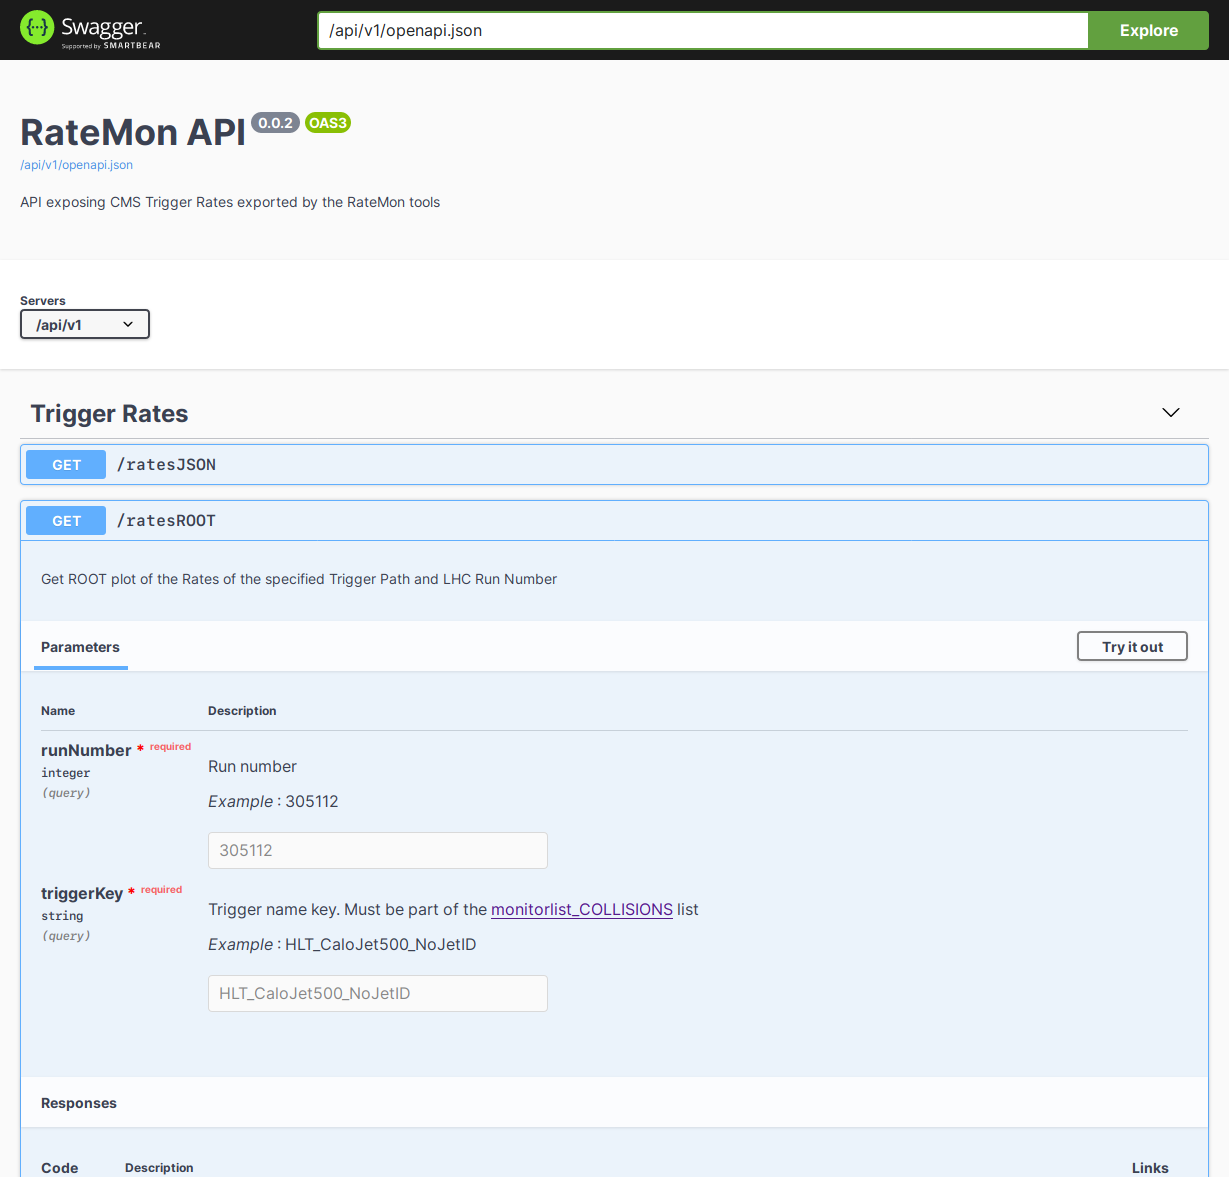
\includegraphics[width=0.8\paperwidth]{figures/swagger-ui}}
    \caption{Swagger UI}
    \label{fig:swagger-ui}
\end{figure}

\subsection{OpenAPI 3 Schema}

\begin{listing}[ht]
\begin{yamlcode}
openapi: "3.0.0"
info:
  version: 0.0.2
  title: RateMon API
  description: API exposing CMS Trigger Rates exported by the RateMon tools
servers:
  - url: http://ater.cern.ch/api/v1
paths:
  /ratesROOT:
    get:
      tags: [Trigger Rates]
      description: |
        Get ROOT plot of the Rates of the specified Trigger Path and LHC Run Number
      operationId: app.getRatesROOT
      parameters:
        - name: runNumber
          in: query
          description: "Run number"
          example: 305112
          required: true
          style: form
          schema:
            type: integer
        - name: triggerKey
          in: query
          description: "Trigger name key. Must be part of the [monitorlist_COLLISIONS](https://gitlab.cern.ch/cms-tsg-fog/ratemon/-/blob/api/ratemon/TriggerLists/monitorlist_COLLISIONS.list) list"
          example: HLT_CaloJet500_NoJetID
          required: true
          schema:
            type: string
      responses:
        '200':
          description: ROOT binary file of the computed plot
\end{yamlcode}
\caption{OpenAPI schema definition of the \texttt{/ratesROOT} API endpoint}
\end{listing}

Connexion, OpenAPI 3 schema, Swagger UI

\subsection{Implementation}

\begin{listing}[ht]
\begin{pythoncode}
def getRatesROOT(runNumber: int, triggerKey: str):
    saveDirectory = "/rtmdata/" + str(runNumber)
    rates = controller.runStandalone(
                         dbConfig=dbCfg,
                         exportRoot=True,
                         saveDirectory=saveDirectory,
                         makeTitle=False,
                         triggerList=[triggerKey],
                         createFit=True,
                         bestFit=True,
                         data_lst=[runNumber])

    return send_from_directory(saveDirectory,
                               triggerKey + '.ROOT',
                               as_attachment=True) # Keep the filename
\end{pythoncode}
\caption{Implementation of the \texttt{/ratesROOT} API endpoint}
\end{listing}

\subsection{Running}
\begin{textcode}
yum install libnsl

export LD_LIBRARY_PATH=/usr/lib/oracle/19.6/client64/lib:LD_LIBRARY_PATH

copy tnsnames.ora

wget https://download.oracle.com/otn_software/linux/instantclient/19600/oracle-instantclient19.6-basic-19.6.0.0.0-1.x86_64.rpm

yum install oracle-instantclient19.6-basic-19.6.0.0.0-1.x86_64.rpm
\end{textcode}

\section{Integration with OMS}

Highcharts, React, Panel

\section{Run Registry}

CMS Run Registry is a in-development tool giving access to a lot of DQM datasets. TODO: describe bug reports, HTTPS auth problems and various contributions done upstream to this tool.


\section{Deployment}

\subsection{Attaching a volume for caching}

To offer more disk space to the caching mechanism, a new volume has been created through the CERN Openstack control panel. Once available, I attached it to the machine serving the RateMon API.

On that machine, \texttt{fdisk -l} will give the disks overview, listing the new volume. I noted the device ID (\texttt{/dev/vdb}) and then executed \texttt{fdisk /dev/vdb} to launch fdisk, the partition manager tool provided by the util-linux standard package.

\begin{textcode}
$ fdisk -l
...
Disk /dev/vdb: 600 GiB, 644245094400 bytes, 1258291200 sectors
Units: sectors of 1 * 512 = 512 bytes
Sector size (logical/physical): 512 bytes / 512 bytes
I/O size (minimum/optimal): 512 bytes / 512 bytes
\end{textcode}

In the fdisk shell, create a new partition (\texttt{n}), select is a primary (\texttt{p}) and denote it as the first (\texttt{1}). Set it to occupy all the available space accepting defaults. Select again the partition (\texttt{t}) and set the Linux partition type (\texttt{83}). (\texttt{p}) displays the partition setup we just defined. If that's okay, (\texttt{w}) commits the modifications and applies them.

\begin{textcode}
Device     Boot Start        End    Sectors  Size Id Type
/dev/vdb1        2048 1258291199 1258289152  600G 83 Linux
\end{textcode}

Back in the standard shell, use \texttt{mkfs.ext4 /dev/vdb} to format the partition using the EXT4 file system.

Note the UUID of our newly formatted partition:

\begin{textcode}
$ mkfs.ext4 /dev/vdb
mke2fs 1.45.4 (23-Sep-2019)
Creating filesystem with 157286400 4k blocks and 39321600 inodes
Filesystem UUID: f74a87c8-7ced-4414-bc62-e09d07be7845
\end{textcode}

Now that we know the UUID, we can mount the volume:

\begin{textcode}
$ mkdir /cache
$ mount /dev/disk/by-uuid/f74a87c8-7ced-4414-bc62-e09d07be7845 /cache
\end{textcode}

To make the mounting persistent, we add this entry to the \texttt{/etc/fstab} file:

\begin{textcode}
UUID=f74a87c8-7ced-4414-bc62-e09d07be7845   /cache  auto defaults,nofail    0 3
\end{textcode}

Here's the final situation, as described by \texttt{df -h}:

\begin{textcode}
$ df -h
Filesystem      Size  Used Avail Use% Mounted on
...
/dev/vda2        40G   33G  7.6G  82% /
/dev/vdb        590G   73M  560G   1% /cache
\end{textcode}

\subsection{NGINX as reverse proxy and cache server}


\begin{textcode}
sudo cat /var/log/audit/audit.log | grep nginx | grep denied
\end{textcode}


\begin{textcode}
$ setsebool -P httpd_can_network_connect 1
\end{textcode}

chown nginx:nginx /cache/

\begin{listing}[ht]
\begin{nginxcode}
# Set cache dir
proxy_cache_path /cache levels=1:2 keys_zone=one:50m max_size=500g inactive=200d;

# Set cache key to include identifying components
proxy_cache_key $scheme$proxy_host$request_uri;

# Add cache status to log
log_format cache '$remote_addr - $remote_user [$time_local] "$request" $status $body_bytes_sent "$http_referer" "$http_user_agent" cs=$upstream_cache_status';

server {
    server_name ater.cern.ch;
    add_header X-Cache-Status $upstream_cache_status;
    
    ## Access and error logs.
    access_log /var/log/nginx/api-proxy.access.log cache;
    error_log  /var/log/nginx/api-cache.error.log;  
    
    location / {
        proxy_set_header Host $host;
        proxy_set_header X-Real-IP $remote_addr;
            
        proxy_cache one;
        proxy_ignore_headers X-Accel-Expires Expires Cache-Control;
        proxy_cache_valid 200 302 200d;
        proxy_cache_valid 404 15m;
        proxy_pass http://localhost:8085;   
    
    }
    listen 80;
}
\end{nginxcode}
\caption{NGINX configuration for reverse proxying and caching}
\end{listing}

\section{A new User Interface}

VueJS, ROOT, Plotly, Plotly -> JSROOT

\begin{figure}
    \centerline{
        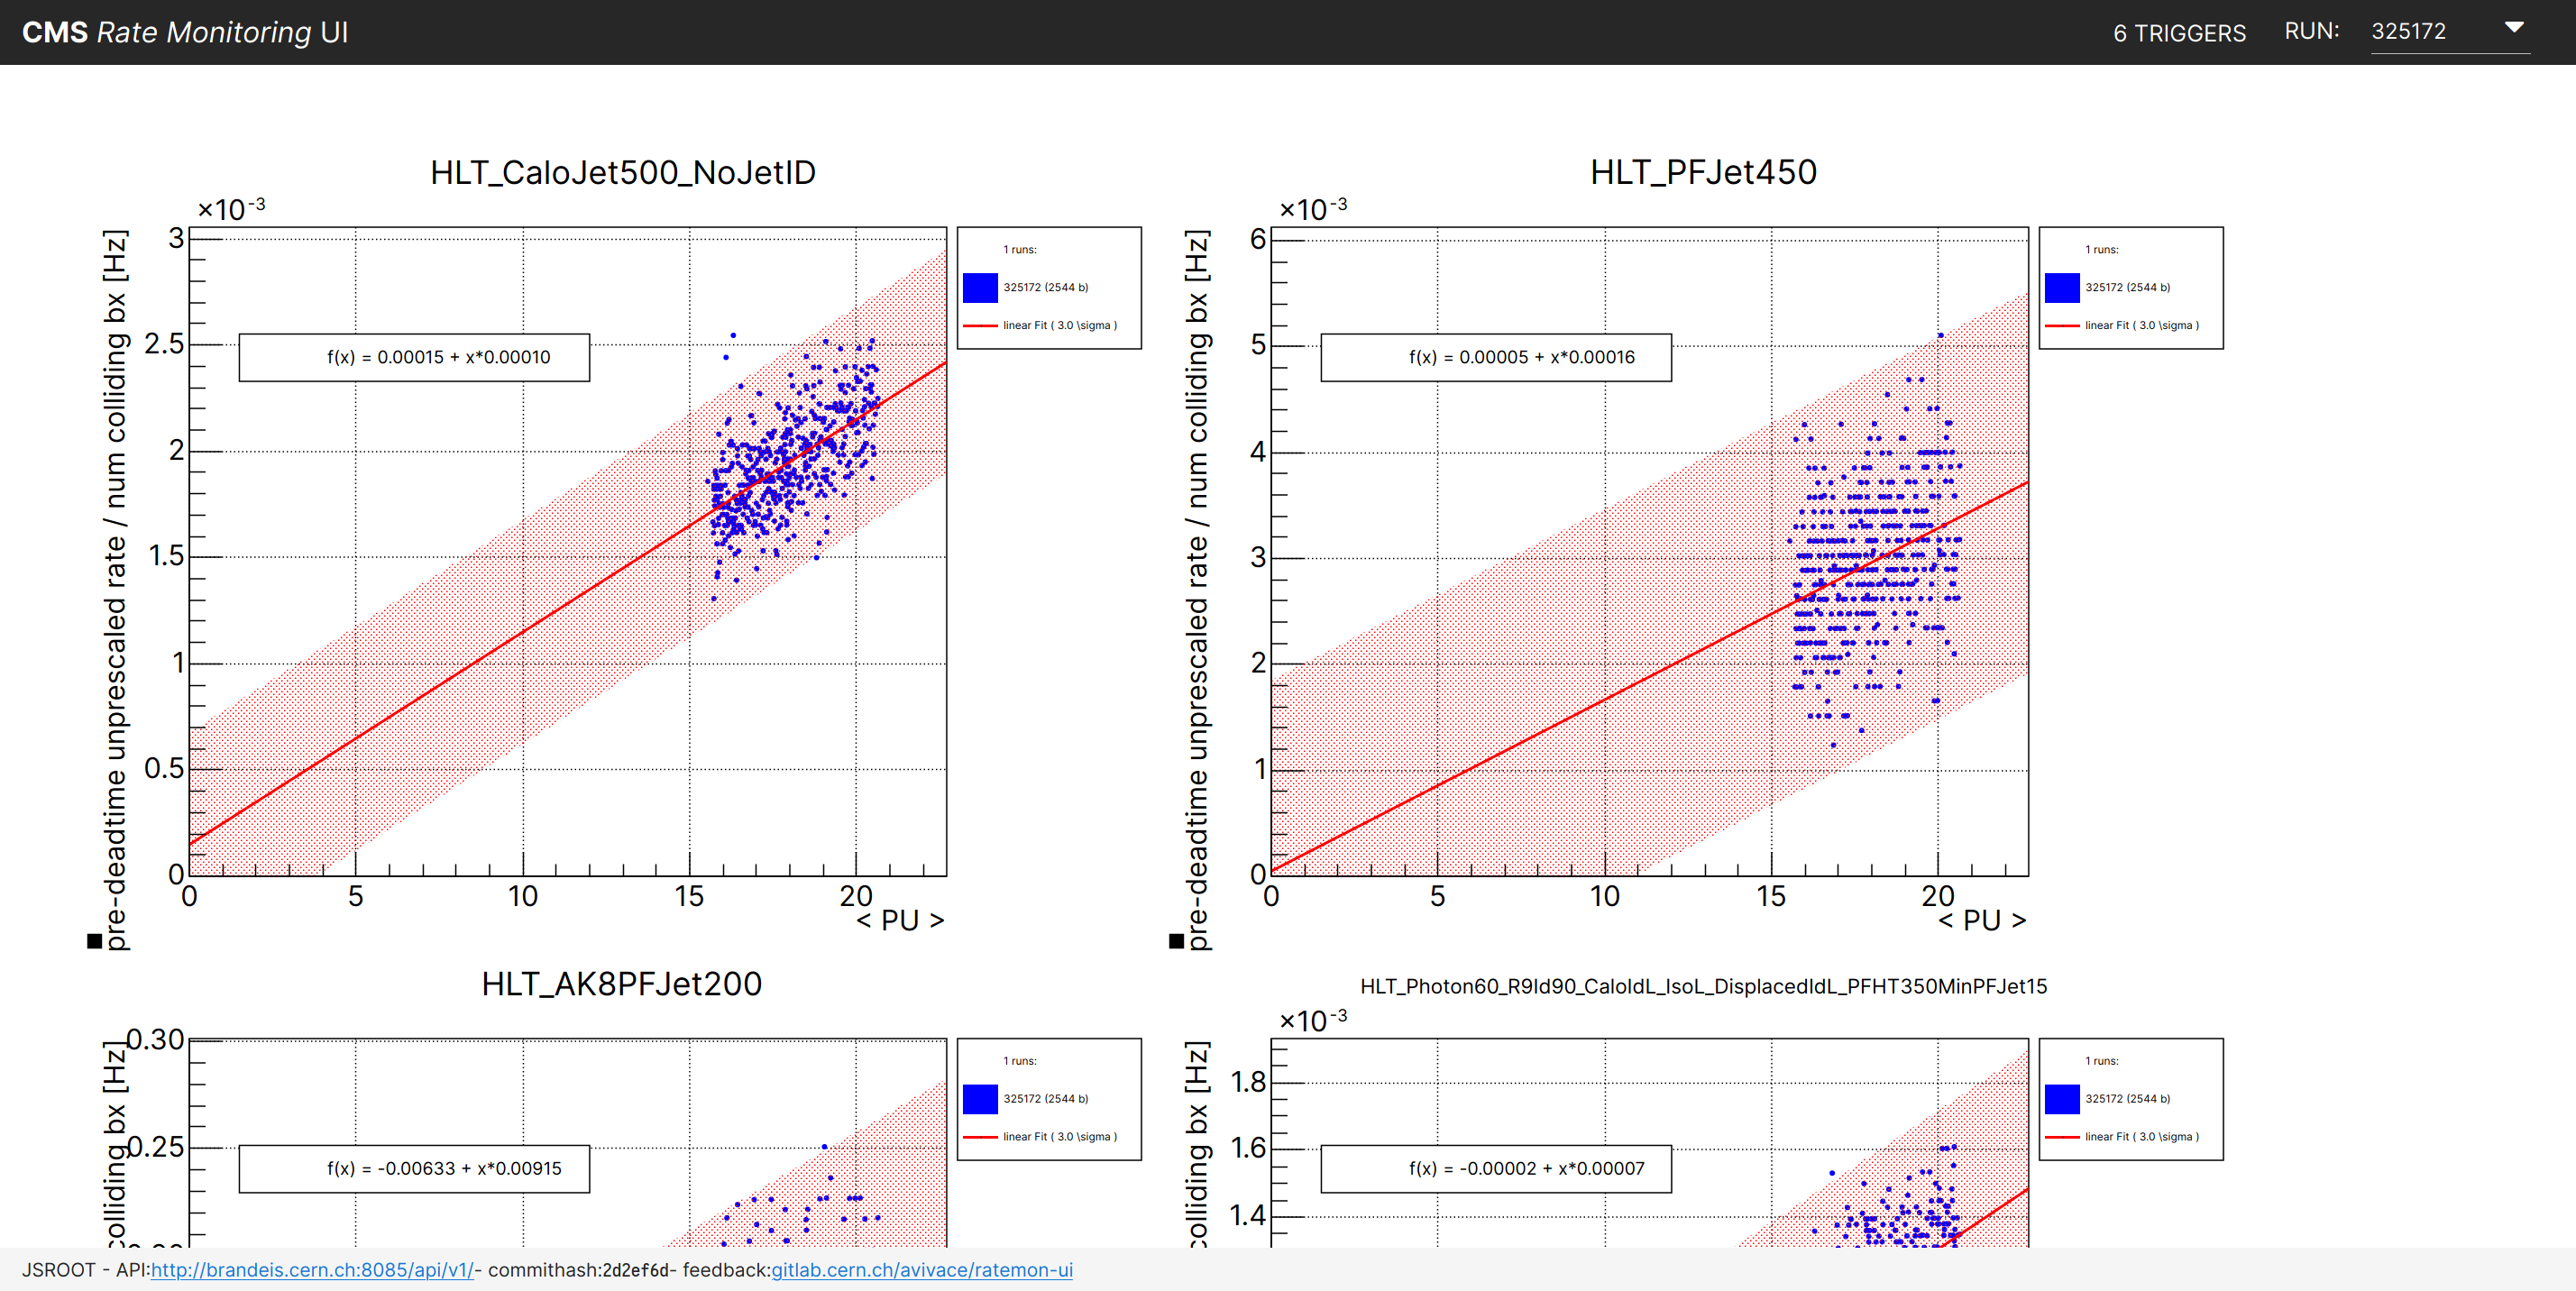
\includegraphics[width=0.9\paperwidth]{figures/ratemon-ui0.png}}
    \caption{Main RateMon UI application view, showing interactive trigger rate plots and relative fit functions}
    \label{fig:ratemon_ui0}
\end{figure}
